\chapter{Discussion}\label{chap:discussion}


%Discuss the results. What is the outcome of your experimetns?

In this secftion we will shortly discuss our results then extensively compare our work to related work, try to make sense out of our results, discuss some challenges faced and finally possible future work. 

\section{Our work}

\section{Related Work}
In this section we will compare - our work to related work, we will first compare us to the baseline model, the original c implementation from Mikolov et al \cite{Mikolov}. We will then compare our self to Gensim, we do this because Gensim allowed us to easily and fastly compute the embeddings, while having access to the loss, and being a python implementaion made everything easier. 

This section will give an overview over 





\subsection{word2vec}
%TODO ask jorg

As mikolov et al. published the original paper about which introduced the SGNS, it is of course releveant to compare ourselves to theim. The first important thing to notice is that Mikolov et al. only trained their model on the very large google news dataset incorporating more than 3 billion words. This makes the comparison of our work more problematic and more of a guessing game. But we will make some assumptions, as they can become interesting. 
In their original paper, Mikolov et al. reported results from 1 and 3. We accord these good results to the very large dataset  and furthermore as a matter of fact their result are better with 3 than with 1 epochs. We do not have any informtaion about the convergence. Hence it would be intersting to use their dataset for comparison. \\
One thing we can compare is the quality of our word embeddings. Mikolov et al. did not report any results on their model with the text8 dataset, but they therefore published their code, and Ji et al \cite{intel} tested the model on the text8 dataset. They reported a similarity of 0.63 on the wordsim task. This is obviously outperformed by all our models. We did not find any explanation on why those results differ as much. \\
The final assumption is that an advanced optimizer could maybe outperform Sgd in terms of quality on a large embedding. This will be discussed in further work.
 


\subsection{Gensim}
Gensim does propose the class w2vec with the following possible parameters\footnote{link to gensim params}, we will describe theim, show our setting, and why we chose the following, we will only describe the prametrs we changed from the default value will be explained, the rest can be found in the appendix. 
They will be presented in the following way: \\
\texttt{name} (type) - \textit{Description} - Value
\begin{itemize}

   \item \texttt{sentences} (iterable of iterables) – Dataset - we used the Original text8 document splitted into sentences of length 20
  \item \texttt{ size }(int) – Dimensionality of the word vectors - 100
\item    \texttt{window} (int) – Maximum distance between the current and predicted word within a sentence - 100
  \item  \texttt{min\_count }(int) – Ignores all words with total frequency lower than this - 5
 \item   \texttt{workers} (int) – Use these many worker threads to train the model (=faster training with multicore machines) - 4 
\item    \texttt{sg} ({0, 1}) – Training algorithm: 1 for skip-gram; otherwise CBOW. -1
  \item  \texttt{hs} ({0, 1}) – If 1, hierarchical softmax will be used for model training. If 0, and negative is non-zero, negative sampling will be used. - 0
  \item  \texttt{negative} (int) – If > 0, negative sampling will be used, the int for negative specifies how many “noise words” should be drawn (usually between 5-20). If set to 0, no negative sampling is used - 10 
\item   \texttt{ ns\_exponent} (float) – Exponent in the unigram distribution, when choosing random samples REFERENCE EQUATION. - 0.75
\item    \texttt{alpha} (float) – The initial learning rate. - 0.025
 \item   \texttt{min\_alpha} (float) – Learning rate will linearly drop to min\_alpha as training progresses. -0.0001

 \item   \texttt{sample} (float) – The threshold for configuring which higher-frequency words are randomly downsampled, useful range is (0, 1e-5). - 1e-4
   \item \texttt{hashfxn} (function) – Hash function to use to randomly initialize weights, for increased training reproducibility. - VERIFY 
  \item  \texttt{iter} (int) – Number of iterations (epochs) over the corpus. - 10 
 \
  \item  \texttt{compute\_loss} (bool) – If True, computes and stores loss value which can be retrieved using get\_latest\_training\_loss(). - True
 \item   \texttt{callbacks} (iterable of CallbackAny2Vec) – Sequence of callbacks to be executed at specific stages during training. - see Appendix
\end{itemize}

\subsubsection{Gensim vs. SGD}
First we have to note that we cannot compare ourselves to gensim in computation time, this woudl not be very smart as our code is written in python and gensim uses advanced cython routines\footnote{link to tutorial thesis}. 
The first interesting thing to note is that we did not have the same values in convergence time as gensim when using sgd. There are differnet possiblilities why this could be the case. First our batched approach could hinder performance in term of convergence as some overwriting may happen. Another differnce between our implementation is the fact that gensim checks whether negative samples are real negative samples. Thererfore the learning of the input and output context is optimized. 
The first hypothesis may be confirmed by the fact that our input shuffling reduces the number of overwritings and therefore we achieved conv time of 7 epcohs which is closer to 4 epochs. and the last difference maybe explained by the eg samples thing. 

\subsubsection{Gensim vs. Adam}
The Adam optimizer did outperform the Gensim application in performance (only slighltlly: 0.01 corr coeff advantage) and convergence time. Adam converged in 2 epochs vs. Gensim in 4. The case to be made here is that one would have to look at the computational advantage to calculate the simple sgd vs.  the adam update rule. Another aspect to look at is that we mainly tested our implementation on the text8 dataset. We only experienced once one the enwik9 dataset. Here the argument that can be made is that, some optimizers work better on specific loss functions in comparison to others, hence we need to show that our optimizer words on amultiued on theim and that it is not just a statistical anomaly.

\begin{figure}[h]
    \centering
			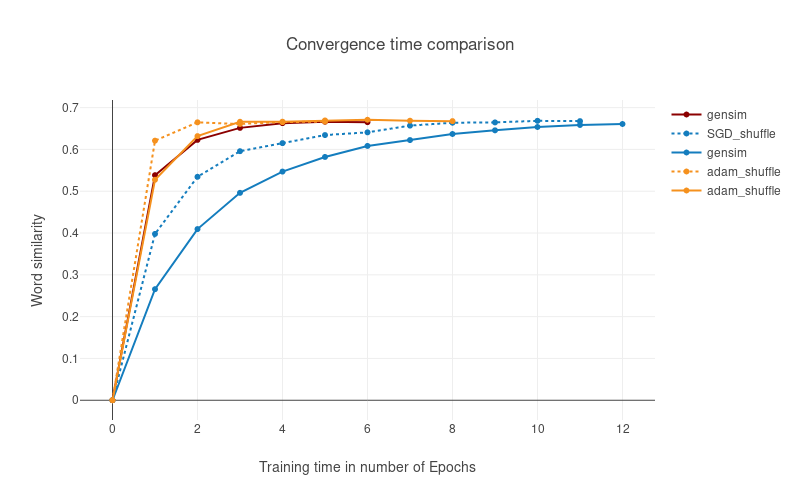
\includegraphics[scale=0.45]{images/gensim_vs_adam} 
    \caption{Training time Stochastic Gradient Descent with input Shuffling}
    \label{fig:gensim_vs_adam}
\end{figure}


\section{Challenges faced}
\subsection{Using the wrong embeddings}
To start our comutation we did choose some wrong, at leat not in coordinance with gensim, initialization embeddings. The context vectors were set between (-1,1) distributed normally. Gensim does it buy putting theim all to 0. As we did the latter the first time our model did not train, but this is possably due to a learning rate that was too low. So we chosed theim to (-1,1). With theim we did not acheive the same similarity as gensim. But when we changed theim back we performed the same results as gensim. Therefore this is a recommendation to future work to not set the initialization to (-1,1)
\subsection{Too big of a batch size}
Another challenge we faced was finding a good batch size. We trained our batch size for a long time with a bs of 5000. But this seemed to worked fine in the beginning but a high lr seemed to work too which was very suspect. We then decided to take a batch size of 2000. Which slightly decreased the learning time, and increased the convergence time and adjusted the learning rate. 
\subsection{Correct loss function}
We expirimented with different loss function as we did not have exactly the same as introduced by mikolov et al. We therefore first ook the average of each score in our tensor. But we then took the sum which seemed to work  better. Is this because the shape of the loss function suits bettter advanced optimizers. Or because it approaches the original loss function more. 


\section{Further Work}
This work only focused on testing the approach of using advanced optimizers and input shuffling to improve the convergence time of the SGNS. While we did show that in theory it could work there dstill needs a bit of work to be done to show that this claim holds consistently. The first thing to do is to use another data set we only tried our approach on only one and a very small dataset. Both of these aspects are problematic. By using a very small dataset we do not use the model in the condition it is mostly needed for as the dataset used in practice a usually 3b words. There is a small argument that can be made for machine translation as the use of small parllel corpus is not unusual . The second one is that some optimizers have shown to perform better on some specific shapes of loss functions. Therefore it could be possible that adam and adagrad only outperform the sgd on this specific loss function for this dataset. Therefore there still needs to be more extensive work done to confirm to confirm our interesting early results. Antoher issue with our implementation is that we didn't care about the throughput of words, so in this matter our implementation is inefficient. One would have to improve one of the already efficient implementation in order to show that we can imporve the convergence time while at the same time maintaining the same convergence time.



